\section{Latex Samples}
\begin{frame}[fragile]
  \frametitle{Latex Samples}
  \begin{itemize}
  \item Bilder (png)
  \item Code Fragmente
  \item Übungen
  \item Theorem
  \item Example
  \end{itemize}
\end{frame}

\begin{frame}[fragile]
  \frametitle{Bilder (png)}
  \centering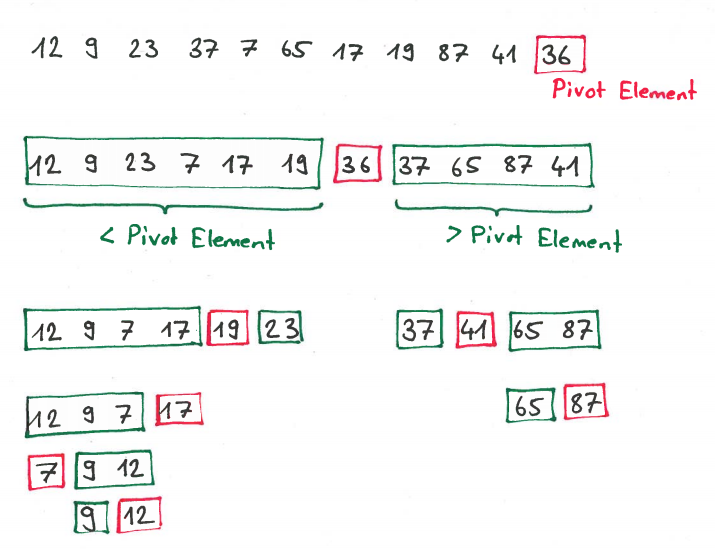
\includegraphics[scale=0.4]{quicksort.png}
\end{frame}

\begin{frame}[fragile]
  \frametitle{Code Fragmente}
  \begin{lstlisting}
  // my first program in C++
  \end{lstlisting}
  \emph{Dies ist eine Kommentar Zeile. Alle Zeilen die mit // beginnen sind
  Kommentare und haben keine Auswirkung auf das Programm. Sie werden
  genutzt um den Code mit Erkl"arungen zu erg"anzen.}
  \vspace{3mm}
  \emph{In C++ existieren zwei M"oglichkeiten f"ur Kommentare:}
  \begin{lstlisting}
  // Dieser Kommentar geht bis ans Ende der Zeile
  /* Dieser Kommentar endet
  beim Erscheinen der Zeichenfolge */
  \end{lstlisting}
\end{frame}

\begin{frame}[fragile]
  \frametitle{Übungen}
  \begin{exercise}
  Das ist eine Übung...
  \end{exercise}
\end{frame}

\begin{frame}[fragile]
  \frametitle{Theorem}
  \begin{theorem}
  Das ist ein Theorem...
  \end{theorem}
\end{frame}

\begin{frame}[fragile]
  \frametitle{Example}
  \begin{example}
  Das ist ein Beispiel...
  \end{example}
\end{frame}
